\chapter{Vector Functions}

\section{Vector Functions and Space Curves}
A vector expression of the form $\ev{f(t),g(t),h(t)}$ is called a vector function.
It can also be described as three separate functions, $x=f(t)$, $y=g(t)$, and $z=h(t)$,
that describe points in space. In this case, we refer to the set of equations as
parametric equations for the curve.
$$r(t)=\ev{f(t),g(t),h(t)}=f(t)\ihat+g(t)\jhat+h(t)\khat$$

\subsection*{Example}
Describe the curves $\ev{cos\:t,sin\:t,0}$, $\ev{cos\:t,sin\:t,t}$, and
$\ev{cos\:t,sin\:t,2t}$

\subsection*{Solution}
As $t$ varies, the first two coordinates in all three functions trace out a unit circle.
In the first curve, the $z$-coordinate is always 0, so this is a 2D unit circle in the
$xy$ plane. In the second curve, the $z$-coordinate varies with $t$ which will
produce a helix. In the third curve, the $z$ coordinate varies twice as fast as $t$
which produces a stretched out helix. Below are the two helixes:
\begin{center}
    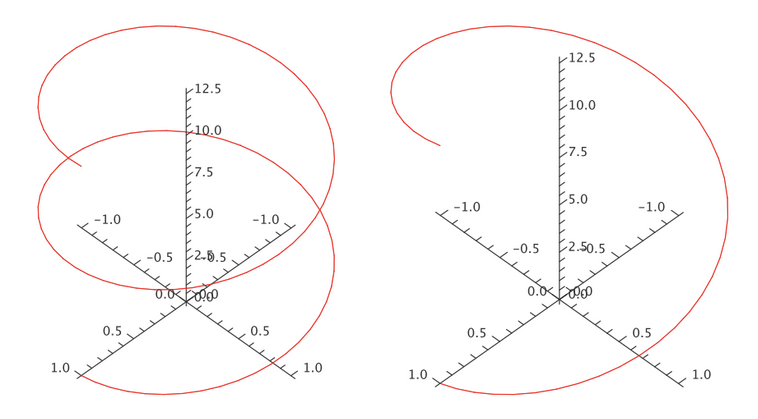
\includegraphics[scale=0.5]{example14-1-1.png}
\end{center}

If $r(t)=\ev{f(t),g(t),h(t)}$, then
$$\lim_{t\to a}r(t)=\ev{\lim_{t\to a}f(t),\lim_{t\to a}g(t),\lim_{t\to a}h(t)}$$
provided the limits of the component functions exist.

\subsection*{Example}
Graph the projections of $\ev{cos\:t,sin\:t,2t}$ onto the $xz$ plane and the $yz$ plane

\subsection*{Solution}
The 2D vector function for the projection onto the $xz$ plane is $\ev{cos\:t,2t}$,
or in parametric force: $x=cos\:t$, $z=2t$. By substituting for $t$, we get
$x=cos(z/2)$, which is the curve below on the left. For the projection onto the $yz$
plane, we start with the vector function $\ev{sin\:t,2t}$, which is $y=sin\:t$,
$z=2t$. Substituting for $t$ gives $y=sin(z/2)$ as shown below on the right.
\begin{center}
    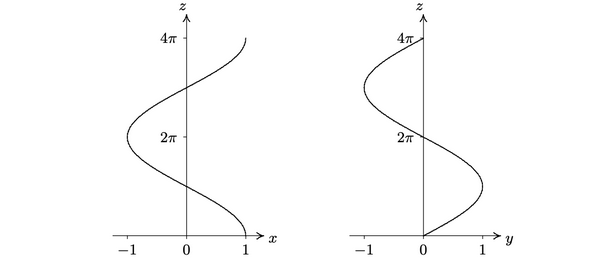
\includegraphics[scale=0.8]{example14-1-2.png}
\end{center}

\section{Derivatives and Integrals of Vector Functions}

\subsection*{Derivatives}
The derivative of a vector function is defined the same way as for real-valued functions:
$$\dv{r}{t}=r'(t)=\lim_{h\to 0}\frac{r(t+h)-r(t)}{h}$$
If $r(t)=\ev{f(t),g(t),h(t)}=f(t)\ihat+g(t)\jhat+h(t)\khat$ where $f$, $g$, and $h$
are differentiable functions, then
$$r'(t)=\ev{f'(t),g'(t),h'(t)}=f'(t)\ihat+g'(t)\jhat+h'(t)\khat$$

\subsection*{Example}
\begin{enumerate}[(a)]
    \item Find the derivative of $r(t)=(1+t^3)\ihat+te^{-t}\jhat+sin\:2t\khat$
    \item Find the unit tangent vector at the point where $t=0$
\end{enumerate}

\subsection*{Solution}
\begin{enumerate}[(a)]
    \item $r'(t)=3t^2\ihat+(1-t)e^{-t}\jhat+2cos\:2t\khat$
    \item Since $r(0)=\ihat$ and $r'(0)=\jhat+2\khat$, the unit tangent vector at
          (1,0,0) is $$T(0)=\frac{r'(0)}{|r'(0)|}=\frac{\jhat+2\khat}{\sqrt{1+4}}=
              \frac{1}{\sqrt{5}}\jhat+\frac{2}{\sqrt{5}}\khat$$
\end{enumerate}

\subsection*{Theorem}
Suppose \textbf{u} and \textbf{v} are differentiable vector functions, $c$ is a scalar,
and $f$ is a real-valued function. Then
\begin{center}
    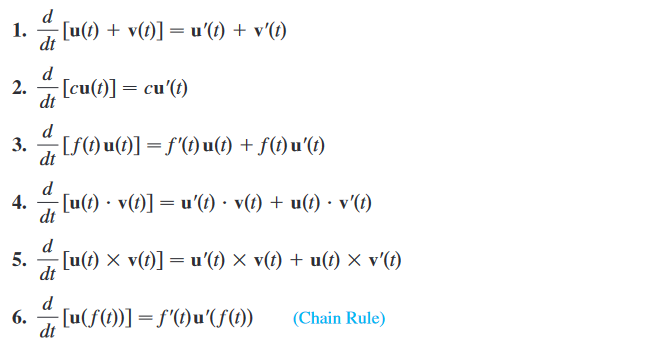
\includegraphics[scale=0.8]{example14-2-1.png}
\end{center}

\subsection*{Integrals}
$$\int_a^b\textbf{r}(t)\:dt=\left(\int_a^bf(t)\:dt\right)\ihat+\left(\int_a^bg(t)\:dt\right)
    \jhat+\left(\int_a^bh(t)\:dt\right)\khat$$

\subsection*{Example}
If $\textbf{r}(t)=2cos\:t\ihat+sin\:t\jhat+2t\khat$, then
\begin{align*}
    \int\textbf{r}(t)\:dt & =\left(\int 2cos\:t\:dt\right)\ihat+\left(\int cos\:t\:dt\right)\jhat+\left(\int 2t\:dt\right)\khat \\
                          & =2sin\:t\ihat-cos\:t\jhat+t^2\khat+C
\end{align*}
Where $C$ is a vector constant of integration, and
$$\int_0^{\pi/2}\textbf{r}(t)\:dt=\left[2sin\:t\ihat-cos\:t\jhat+t^2\khat\right]_0^{\pi/2}=
    2\ihat+\jhat+\frac{\pi^2}{4}\khat$$

\section{Arc Length and Curvature}

\subsection*{Length of a Curve}
$$L=\int_a^b\sqrt{[f'(t)]^2+[g'(t)]^2+[h'(t)]^2}\:dt$$
$$=\int_a^b\sqrt{(\dv{x}{t})^2+(\dv{y}{t})^2+(\dv{z}{t})^2}\:dt$$
The formula can be put into the compact form $L=\int_a^b|\textbf{r}'(t)|\:dt$

\subsection*{Example}
Find the length of the arc of the circular helix with vector equation
$\textbf{r}(t)=\cos{t}\ihat+\sin{t}\jhat+t\khat$ from the point $(1,0,0)$ to the
point $(1,0,2\pi)$

\subsection*{Solution}
Since $\textbf{r}'(t)=-\sin{t}\ihat+\cos{t}\jhat+\khat$, we have
$$|\textbf{r}'(t)|=\sqrt{(-\sin{t})^2+cos^2t+1}=\sqrt{2}$$
The arc from (1,0,0) to (1,0,$2\pi$) is described by the parameter interval
$0\leq t\leq 2\pi$ and so we have
$$L=\int_0^{2\pi}|\textbf{r}'(t)|\:dt=\int_0^{2\pi}\sqrt{2}\:dt=2\sqrt{2}\pi$$

\subsection*{Proof}
$$\kappa=\left|\dv{\textbf{T}}{s}\right|\to\dv{\textbf{T}}{t}=
    \dv{\textbf{T}}{s}\dv{s}{t}$$
$$\kappa=\frac{|d\textbf{T}/dt|}{|ds/dt|}$$
$$\kappa(t)=\frac{|\textbf{T}'(t)|}{|\textbf{r}'(t)|}
    =\frac{|\textbf{r}'(t)\times\textbf{r}''(t)|}{|\textbf{r}'(t)|^3}$$

We summarize here the formulas for unit tangent, unit normal and binormal vectors,
and curvature.
$$\textbf{T}(t)=\frac{\textbf{r}'(t)}{|\textbf{r}'(t)|} \qquad
    \textbf{N}(t)=\frac{\textbf{T}'(t)}{|\textbf{T}'(t)|} \qquad
    \textbf{B}(t)=\textbf{T}(t)\times\textbf{N}(t)$$
$$\kappa=|\dv{\textbf{T}}{s}|=\frac{|\textbf{T}'(t)|}{|\textbf{r}'(t)|}
    =\frac{|\textbf{r}'(t)\times\textbf{r}''(t)|}{|\textbf{r}'(t)|^3}$$

\section{Motion in Space: Velocity and Acceleration}
Suppose a particle moves through space so that its position vector at time $t$ is
$\textbf{r}(t)$. Notice that for small values of $h$, the vector
$$\frac{\textbf{r}(t+h)-\textbf{r}(t)}{h}$$
approximates the direction of the particle moving along the curve $\textbf{r}(t)$.
Its magnitude measures the size of the displacement vector per unit time. The vector
gives the average velocity over a time interval of length and its limit is the
\textbf{velocity vector} $\textbf{v}(t)$ at time $t$:
$$\textbf{v}(t)=\lim_{h\to 0}\frac{\textbf{r}(t+h)-\textbf{r}(t)}{h}=\textbf{r}'(t)$$

\subsection*{Example}
The position vector of an object moving in a place is given by $\textbf{r}(t)=
    t^3\ihat+t^2\jhat$. Find its velocity, speed, and acceleration when $t=1$.

\subsection*{Solution}
The velocity and acceleration equations at time $t$ are
$$\textbf{v}(t)=\textbf{r}'(t)=3t^2\ihat+2t\jhat$$
$$\textbf{a}(t)=\textbf{r}''(t)=6t\ihat+2\jhat$$
and the speed is
$$|\textbf{v}(t)|=\sqrt{(3t^2)^2+(2t)^2}=\sqrt{9t^4+4t^2}$$
When $t=1$, we have
$$\textbf{v}(1)=3\ihat+2\jhat\qquad\textbf{a}(1)=6\ihat+2\jhat\qquad|\textbf{v}(1)|=\sqrt{13}$$

\subsection*{Parametric Equations of Trajectory}
$$x=(v_0\cos{\alpha})t\qquad y=(v_0\sin{\alpha})t=\frac{1}{2}gt^2$$

\subsection*{Tangential and Normal Components of Acceleration}
$$\textbf{T}(t)=\frac{\textbf{v}}{v} \qquad \textbf{v}=v\textbf{T}$$
$$\textbf{a}=\textbf{v}'=v'\textbf{T}+v\textbf{T}'$$
$$\kappa=\mathbf{\cfrac{|T'|}{|r'|}}=\cfrac{|\textbf{T}'|}{v} \qquad
    |\textbf{T}'|=\kappa v$$
$$\textbf{N}=\mathbf{\frac{T'}{|T'|}}\qquad \mathbf{T'=|T'|N=\kappa}v\textbf{N}$$
$$\textbf{a}=v'\textbf{T}+\kappa v^2 \textbf{N}$$

\subsection*{Keplar's Laws}
\begin{enumerate}
    \item A planet revolves around the Sun in an elliptical orbit with the Sun at one focus.
    \item The line joining the Sun to a planet sweeps out equal areas in equal times.
    \item The square of the period of revolution of a planet is proportional to the cube
          of the length of the major axis of its orbit.
\end{enumerate}